\chapter{Metodología}\label{cap:3}
\lettrine{P}{ara modelar el proceso de amplificación} de la semilla de armónicos de alto orden introducida a través del canal de plasma, es necesario plantear y resolver numéricamente las denominadas en la literatura como ecuaciones de Maxwell-Bloch o \emph{\acrfull{mbe}}. El código Dagon empleado durante las simulaciones implementa estas ecuaciones mediante un programa escrito en Fortran que, a su vez, está acoplado con otros códigos numéricos (cuya función se explicará más detalladamente en la sección \S\ref{sec:3.2}), recibiendo información de partida para iniciar el procedimiento de cálculo. De esta forma, los resultados proporcionan los datos necesarios para comprender cómo afectan la densidad de iones y electrones libres en el plasma a la intensidad y perfil de fase del haz \acrshort{xuv} obtenido. 

Una vez finalizadas las simulaciones, para poder realizar el análisis de las imágenes y los resultados obtenidos, se emplearon dos nuevos programas ---esta vez escritos en Python y GNU Octave---, que permiten almacenar los datos obtenidos en las simulaciones de Dagon y representarlos gráficamente mediante curvas bidimensionales. Además, estos conjuntos de datos pueden introducirse en programas como VisIt para la construcción de imágenes tridimensionales y bidimensionales, por ejemplo, de la propagación del \acrshort{hoh} en la dirección longitudinal del canal.

\section{Ecuaciones de Maxwell-Bloch}\label{sec:3.1}
En este trabajo, el fenómeno físico de la amplificación del armónico inyectado en el plasma de iones de kriptón conduce inevitablemente hasta estas ecuaciones, puesto que determinan cuáles serán las propiedades de la emisión obtenida. Las \acrshort{mbe} describen la dinámica de la interacción entre los modos de vibración de un campo electromagnético y los átomos de un sistema cuántico con dos estados posibles: el estado base $\ket{1}$, y el estado excitado $\ket{2}$. 

El formalismo físico-matemático utilizado en mecánica cuántica para obtener las ecuaciones no es trivial\autocite{Cohen-Tannoudji2019a,Sakurai2020,Milonni1988}, aunque tiene la ventaja de predecir con suficiente exactitud la evolución temporal del pulso, además de propiedades físicas de los fotones como su \acrshort{oam}, mientras que otros métodos más sencillos ---como el programa de trazado de rayos SHADOX--- no ofrecen esta opción, si bien podría utilizarse para resolver el problema de la amplificación en el plasma. 

En la interacción láser-plasma estudiada, para obtener una buena aproximación basta considerar el campo eléctrico $\symbfcal{E}$ de la semilla \acrshort{hoh}, aunque cálculos más precisos tendrían que incorporar el acoplamiento del campo magnético $\symbfcal{B}$. Además, el acoplamiento entre el campo electromagnético y la materia utiliza una aproximación semiclásica, donde los átomos o iones son sistemas cuánticos de dos estados descritos por la ecuación de Schrödinger, mientras que la luz es un sistema clásico ---una onda electromagnética--- descrito por las ecuaciones de Maxwell. 

En primer lugar, el acoplamiento del campo eléctrico con el plasma es la ecuación de ondas 
\begin{equation}\label{eq:3.0}
  \laplacian \symbfcal{E} - \frac{1}{c^{2}}\pdvN{\symbfcal{E}}{t}{2} = \frac{\omega^{2}_{pe}}{c^{2}}\symbfcal{E} + \frac{1}{\epsilon_{0}c^{2}}\pdvN{\symbfcal{P}}{t}{2},
\end{equation}
donde, como aparecía mostrado en la sección \S\ref{sec:1.2.2}, el campo eléctrico $\symbfcal{E}$, la polarización $\symbfcal{P}$, la frecuencia de las oscilaciones del plasma $\omega_{pe}$ y la constante dieléctrica $\epsilon_{0}$ son función del espacio y del tiempo. 

Como primera hipótesis, se considera la llamada en óptica\autocite{Born2019} como \emph{aproximación paraxial} del campo eléctrico según la dirección de propagación escogida, en este caso, el eje $z$. Sin pérdida de generalidad ---escogiendo un sistema de referencia adecuado---, suponiendo que la radiación está polarizada linealmente según el eje $x$, esta hipótesis permite tener en cuenta únicamente dicha componente del campo eléctrico y de la polarización \autocite{Larroche2000}, dirección en la que oscilarían ambos campos. Las soluciones pueden escribirse separando la envolvente y las vibraciones como
\begin{align}
  \label{eq:3.1a}
  \symcal{E}_{x}(\symbf{r},t) &= \RE \left[E_{R}(\symbf{r},t)\eu^{\iu (kz - \omega t)} + E_{L}(\symbf{r},t)\eu^{\iu (kz + \omega t)}\right], \\
  \label{eq:3.1b}
  \symcal{P}_{x}(\symbf{r},t) &= \RE \left[P_{R}(\symbf{r},t)\eu^{\iu (kz - \omega t)} + P_{L}(\symbf{r},t)\eu^{\iu (kz + \omega t)}\right], 
\end{align}
donde $E_{R}$, $E_{L}$, $P_{R}$, $P_{L}$ son la amplitud de las oscilaciones de las ondas viajeras hacia la dirección positiva y negativa del eje $z$, respectivamente. 

Combinando las ecuaciones \eqref{eq:3.0} y \eqref{eq:3.1a}, y \enquote{agrupando} las componentes que se propagan a lo largo de todo el eje $z$, se obtiene para el campo eléctrico
\begin{align}
  \laplacian \symcal{E}_{x} 
  &= 
  \RE \Bigg[\left(\pdvN{E_{LR}}{x}{2} + \pdvN{E_{LR}}{y}{2} + \pdvN{E_{LR}}{z}{2} + 2k \iu \pdv{E_{LR}}{z} - k^{2}E_{LR}\right)\eu^{\iu (kz \mp \omega t)}\Bigg], \\
  \pdvN{\symcal{E}_{x}}{t}{2}
  &= 
  \RE \Bigg[\left(\pdvN{E_{LR}}{t}{2} \mp 2 \omega \iu \pdv{E_{LR}}{t} - \omega^{2}E_{LR}\right)\eu^{\iu (kz \mp \omega t)}\Bigg],
\end{align}
obteniéndose el lado izquierdo ($\mathrm{LHS}$) de la ecuación de ondas para el campo eléctrico
\begin{equation}\label{eq:3.2}
  \begin{split}
    \mathrm{LHS} = \RE \Bigg[\bigg(\laplacian_{\perp}E_{LR} &+ \pdvN{E_{LR}}{z}{2} + 2k \iu \pdv{E_{LR}}{z} - \frac{1}{c^{2}}\bigg(\pdvN{E_{LR}}{t}{2} \pm 2 \omega \iu \pdv{E_{LR}}{z}\bigg) \\
      &+  \bigg(\frac{\omega^{2}}{c^{2}} - k^{2}\bigg)E_{LR}\bigg)\eu^{\iu(kz \mp \omega t)}\Bigg],
  \end{split}
\end{equation}
donde $\laplacian_{\perp}$ contiene las derivadas de segundo orden en las variables $x, y$ del laplaciano $\laplacian $.

Continuando con la segunda hipótesis, es importante considerar la aproximación de la envolvente lentamente variable o \emph{\acrfull{svea}} que asume la variación temporal y espacial de la envolvente lenta\autocite{Larroche2000} comparada con su longitud de onda, de manera que ambas envolventes del campo eléctrico y polarización verifican
\begin{equation}\label{eq:3.3}
  \abs{\pdvN{A}{z}{2}} \ll \abs{k \pdv{A}{z}}, \quad \abs{\pdvN{A}{t}{2}} \ll \abs{\omega \pdv{A}{t}},
\end{equation}
con $A$ la envolvente de las ondas solución de la ecuación \eqref{eq:3.0}. 

La ecuación \eqref{eq:3.2} puede reducirse más simplificando la relación de dispersión del campo eléctrico en el plasma $\omega^{2} = \omega^{2}_{pe} + k^{2}c^{2}\approx k^{2}c^{2}$, puesto que para la emisión de radiación \acrshort{xuv} o rayos X blandos $\lambda<\qty{40}{nm}$ y la densidad electrónica del plasma de kriptón $n_e<\qty{e21}{cm^{-3}}$ se tiene que, por un lado, $\omega_{pe}=n_{e}e^{2}/\epsilon_{0}m_{e}<\qty{1,8e15}{rad/s}$ y, por otra parte, $kc=2 \pi c/\lambda>\qty{4,7e16}{rad/s}$, entonces $\omega^{2} \gg \omega_{pe}^{2}$ y la aproximación de la relación de dispersión estaría justificada, ya que ambos términos difieren como mínimo en dos órdenes de magnitud. 

Para señalar la importancia del concepto de la \acrshort{svea} en la resolución de las \acrshort{mbe} mediante cualquier método numérico, la Figura \ref{fig:3.1} muestra esquemáticamente un pulso cuya envolvente ---del campo eléctrico--- varía lentamente, propagándose en la dirección $z$.

\begin{figure}[htbp]
  \centering
  \begin{subcaptionblock}{.4\textwidth}
    \centering
    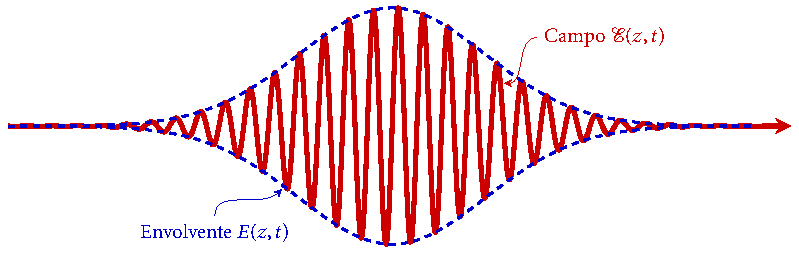
\includegraphics[width=1.1\textwidth]{Figuras/ch3_pulso2d.pdf}
    \caption{Pulso 2D}\label{fig:3.1a}
  \end{subcaptionblock}%
  \begin{subcaptionblock}{.4\textwidth}
    \centering
    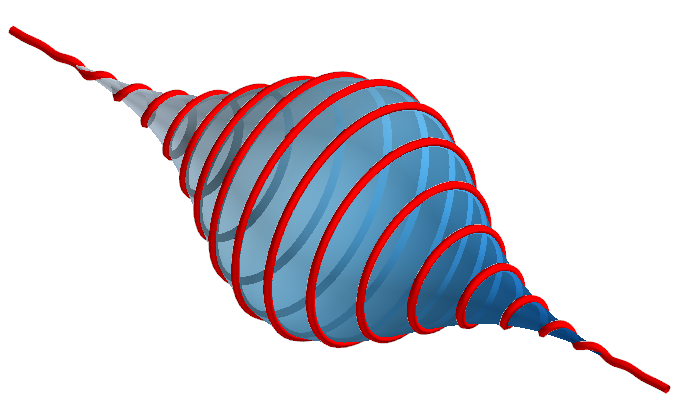
\includegraphics[width=0.8\textwidth]{Figuras/ch3_pulso3d.png}
    \caption{Pulso 3D}\label{fig:3.1b}
  \end{subcaptionblock}%
  \caption{Representación 2D  y 3D  de un pulso láser con la aproximación \acrshort{svea}.}
  \label{fig:3.1}
\end{figure}

A modo ilustrativo, la Figura \ref{fig:3.1b} del pulso tridimensional ha sido elaborada mediante la escritura del Código \ref{cod:3.1} que recurre a la librería Mayavi de Python para su representación.

\begin{listing}[htbp!]
  \caption{Código escrito para representar una \acrshort{svea} de un pulso 3D.}
  \inputminted[firstline=1, lastline=33]{python}{Programas/mlaser.py}
  \label{cod:3.1}
\end{listing}

Empleando las aproximaciones para la relación de dispersión y la envolvente del campo eléctrico consideradas, la ecuación \eqref{eq:3.2} finalmente queda
\begin{equation}\label{eq:3.4}
  \mathrm{LHS} =
  \RE \Bigg[\left(\laplacian_{\perp}E_{LR} + \frac{2 \omega \iu }{c^{2}} \left(\pdv{E_{LR}}{t} \pm c \pdv{E_{LR}}{z}\right)\right)\eu^{\iu (kz \mp \omega t)}\Bigg].
\end{equation}

En segundo lugar, el lado derecho ($\symrm{RHS}$) de la ecuación \eqref{eq:3.0} contiene el término para la polarización del plasma, cuya descomposición en ondas viajeras mostraba la ecuación \eqref{eq:3.1b}, obteniéndose que
\begin{equation}\label{eq:3.5}
  \pdvN{\symcal{P}_{x}}{t}{2} = 
  \RE \Bigg[\left(\pdvN{P_{LR}}{t}{2} \mp 2 \omega \iu \pdv{P_{LR}}{z} - \omega^{2}P_{LR}\right)\eu^{\iu (kz \mp \omega t)}\Bigg].
\end{equation}
Recordando la aproximación \acrshort{svea} de las ecuaciones \eqref{eq:3.4} para las envolventes, junto a la relación de dispersión $\omega^{2} \approx k^{2}c^{2}$, puede considerarse que la amplitud de la polarización en un periodo de onda $\omega$ es mucho mayor que la variación temporal de su envolvente, es decir,
\begin{equation}
  \abs{\pdv{P_{LR}}{t}} \ll \abs{\omega P_{LR}},
\end{equation}
quedando la ecuación \eqref{eq:3.5} como
\begin{equation}\label{eq:3.6}
  \pdvN{\symcal{P}_{x}}{t}{2} = \RE \left[- \omega^{2}P_{LR}\eu^{\iu (\omega t \pm kz)}\right].
\end{equation}
Por último, la sustitución de las ecuaciones \eqref{eq:3.4} y \eqref{eq:3.6} en la ecuación \eqref{eq:3.0} permite obtener, tras reagrupar los términos a izquierda ($\symrm{LHS}$) y derecha ($\symrm{RHS}$), respectivamente
\begin{equation}\label{eq:3.7}
  \tcboxmath{\pdv{E_{LR}}{t} \pm c \pdv{E_{LR}}{z} = \frac{\iu c^{2}}{2 \omega}\laplacian_{\perp}E_{LR} + \frac{\iu \omega}{2} \left[\mu_{0}c^{2}P_{LR} - \left(\frac{\omega_{pe}}{\omega}\right)^{2}E_{LR}\right],}
\end{equation}
obteniendo una ecuación en derivadas parciales de segundo orden en el espacio y primer orden en el tiempo con un término fuente $P_{LR}$ función de las coordenadas espaciales y temporales. 

Es importante señalar que el subíndice $LR$ utilizado representa una forma reducida de escribir las ondas viajeras en sentido positivo $R$ y negativo $L$ del eje $z$. La ecuación de ondas \eqref{eq:3.0} es lineal, cumpliéndose el principio de superposición y, por tanto, la combinación lineal de ondas utilizada es la solución completa de la ecuación. Expandiendo la ecuación \eqref{eq:3.8}, cada solución debe cumplir
\begin{align}
  \pdv{E_{R}}{t} + c \pdv{E_{R}}{z} &= \frac{\iu c^{2}}{2 \omega}\laplacian_{\perp}E_{R} + \frac{\iu \omega}{2} \left[\mu_{0}c^{2}P_{R} - \left(\frac{\omega_{pe}}{\omega}\right)^{2}E_{R}\right], \\
  \pdv{E_{L}}{t} - c \pdv{E_{L}}{z} &= \frac{\iu c^{2}}{2 \omega}\laplacian_{\perp}E_{L} + \frac{\iu \omega}{2} \left[\mu_{0}c^{2}P_{L} - \left(\frac{\omega_{pe}}{\omega}\right)^{2}E_{L}\right],
\end{align}
cuya suma proporciona la ecuación \eqref{eq:3.7}, empleando la notación compacta sugerida.

Hasta este momento, el marco teórico utilizado para el tratamiento de la radiación ha sido clásico, pero como se ha explicado al principio de este sección \S\ref{sec:3.1}, la teoría electromagnética clásica no proporciona una descripción satisfactoria \autocite{Griffiths2017} de la interacción entre la luz y la materia a estas escalas, siendo necesario cuantizar el comportamiento de la materia para comprender la polarización resultante.

Por tanto, hay que introducir una ecuación constitutiva que relacione la naturaleza de la interacción entre la luz (el campo eléctrico), y la materia (la polarización). En la teoría cuántica, la relación \autocite{Cohen-Tannoudji2019} viene dada por
\begin{equation}\label{eq:3.8}
  P = \xval{D} = \symrm{Tr} \left(\rho D \right),
\end{equation}
donde $\rho$ es el operador de densidad, $D$ el operador momento dipolar eléctrico atómico y $\symrm{Tr}$ representa la traza (suma de los elementos de la diagonal principal) del producto de ambos operadores, expresados como matrices en una base ortonormal $\left\{\ket{u_{i}(\symbf{r})}\right\}_{i \in \symbb{N}} \in \symcal{F}$, siendo $\symcal{F}$ un subespacio vectorial \autocite{Cohen-Tannoudji2019} formado por funciones suficientemente regulares para estudiar la amplificación. Empleando como base los estados $\ket{1}$ y $\ket{2}$ del sistema (que están normalizados a la unidad), la matriz de densidad puede representarse como
\begin{equation}\label{eq:3.9}
  \rho(\symbf{r},t) \doteq  
  \begin{pmatrix}
    \rho_{11}(\symbf{r},t) & \rho_{12}(\symbf{r},t) \\
    \rho_{21}(\symbf{r},t) & \rho_{22}(\symbf{r},t)
  \end{pmatrix},
\end{equation}
donde el símbolo $\doteq $ significa \enquote{está representado por}.

Con el objetivo de aportar mayor claridad en la discusión cuántica de la polarización, es necesario realizar una breve explicación de los conceptos introducidos y su significado. El plasma objeto de estudio puede aproximarse \autocite{Milonni1988} como un sistema de dos estados puros $\ket{1}$ y $\ket{2}$ posibles linealmente independientes \autocite{Cohen-Tannoudji2019}, de manera que la probabilidad de encontrarse en cualquiera de ambos estados es $p_{1} + p_{2} = 1$.

En este contexto, el momento dipolar eléctrico $D$ es el observable que se desea medir, y la polarización $P$ es su valor esperado. El operador de densidad es particularmente importante en sistemas donde no se conoce (o es imposible conocer) la totalidad de la información sobre el estado inicial del sistema ---los iones y electrones del plasma en este caso---, ni tampoco pueden determinarse con total precisión los resultados de las mediciones debido a la naturaleza probabilística de los sistemas cuánticos. 

Ambos estados, pertenecientes al espacio vectorial $\symcal{F}$, pueden emplearse como una base ortonormal, pues como se ha comentado anteriormente, son linealmente independientes y están normalizados a la unidad, de tal forma que en el caso más general posible, el estado del sistema consiste en una superposición de ambos estados
\begin{align}
  \ket{\Psi} = c_{1}\ket{1} + c_{2}\ket{2} &= \sum_{k} c_{k}\ket{k}, \\
  \abs{c_{1}}^{2} + \abs{c_{2}}^{2} &= 1,
\end{align}
con $k \in \{1,2\}$ un subíndice para designar cualquiera de los dos estados posibles. La combinación lineal de estos estados implica que los elementos $\rho_{nn}$ y $\rho_{nm}$ de la matriz de densidad pueden escribirse como
\begin{equation}\label{eq:3.10}
  \rho_{nn} = \abs{c_{n}}^{2}, \quad 
  \rho_{nm} = c_{n}c^{*}_{m}
\end{equation}
donde $\abs{c_{n}}^{2}$ es un número real positivo que representa la probabilidad, en una medición del sistema en el estado superpuesto $\ket{\Psi}$, de encontrarlo en el estado $\ket{n}$. Por otro lado, los términos cruzados de la forma $c_{n}c^{*}_{m}$ expresan el fenómeno de interferencia que puede aparecer entre dos estados $\ket{n}$ y $\ket{m}$ cuando el estado $\ket{\Psi}$ es una combinación lineal de los anteriores, como ocurre en este modelo. 

Observando la ecuación \eqref{eq:3.10}, está claro que $\rho_{nn}$ es cero solamente si los $c_{n}$ son cero, mientras que $\rho_{nm}$ puede ser cero cuando alguno (o los dos) de los términos cruzados $c_{n}$ o $c^{*}_{m}$ son cero, siendo estos números complejos. Por lo tanto, si $\rho_{nm}$ es cero significa que los efectos de interferencia entre los estados $\ket{n}$ y $\ket{m}$ han desaparecido, mientras que si $\rho_{nm}$ es distinto de cero entonces persiste una cierta \enquote{coherencia} entre ambos estados, motivo por el cual los elementos fuera de la diagonal $\rho_{nm}$ son llamados \emph{coherencias}.

A raíz de esta exposición, las entradas de la matriz de densidad tienen el siguiente significado: los elementos en la diagonal principal $\rho_{nn}$ representan la probabilidad media de encontrar el sistema en el estado $\ket{n}$, motivo por el que se conocen como las \emph{poblaciones} del estado $\ket{n}$, ya que para un número elevado $N$ de mediciones de la misma propiedad, bajo las mismas condiciones iniciales, $N \rho_{nn}$ sistemas estarán en el estado $\ket{n}$. En cambio, $\rho_{nm}$ es la coherencia entre los dos niveles atómicos del plasma, luego está relacionado con la capacidad del campo eléctrico $\symcal{E}$ del \acrshort{hoh} de provocar la polarización de las partículas que lo constituyen.

Es posible demostrar \autocite{Cohen-Tannoudji2019} que el conocimiento de la matriz de densidad es suficiente para caracterizar el sistema cuántico, empleando la ecuación de Schrödinger (Bloch)
\begin{equation}\label{eq:3.11}
  i \hslash \pdv{\rho(\symbf{r},t)}{t} = \left[H,\rho\right],
\end{equation}
con $H(\symbf{r},t) = H_{0} + W(\symbf{r},t)$, siendo $H_{a}$ el operador Hamiltoniano atómico, $W = -\symbfcal{D} \cdot \symbfcal{E}(\symbf{r},t)$ el potencial electrostático que encierra la interacción entre el campo eléctrico $\symbfcal{E}$ y los estados del sistema, y $\left[H, \rho\right] = H \rho - \rho H$ el conmutador de ambos operadores. Esta expansión del Hamiltoniano es conocida como \emph{aproximación dipolar} \autocite{Jackson1998} y es válida cuando la longitud de onda de la radiación emitida ---rayos X blandos en este caso--- es considerablemente superior que el tamaño promedio del átomo estudiado ($\lambda \sim \qty{10}{nm}$ frente a $R_{a} \sim \qty{0.1}{nm}$ de radio atómico). 

En realidad, el operador momento dipolar eléctrico $D$ puede escribirse como $D = -e \hat{r}_{a}$, siendo $\hat{r}_{a}$ el operador posición relativa entre el núcleo atómico y el electrón, y $e$ la carga eléctrica del electrón. Esto significa que puede representarse como un vector $\symbfcal{D}$ cuyos componentes son los elementos fuera de la diagonal principal de la matriz dipolar asociada, ya que $D$ representa el momento dipolar eléctrico asociado a la transición entre estados ---que naturalmente son diferentes---, y por tanto, los elementos de la diagonal principal tienen que ser cero. Debido a esto, el potencial de interacción puede ponerse como
\begin{equation}
  W = -\symbfcal{D} \cdot \symbfcal{E} =  
  \begin{pmatrix}
    0 & d_{12}\symcal{E}_{x} \\
    d_{21}\symcal{E}_{x} & 0 
  \end{pmatrix} \triangleq
  \begin{pmatrix}
    d_{12}\symcal{E}_{x} \\
    d_{21}\symcal{E}_{x}
  \end{pmatrix} 
  =
  \begin{pmatrix}
    d_{12} \\
    d_{21}
  \end{pmatrix}
  \symcal{E}_{x},
\end{equation}
con el símbolo $\triangleq$ tomando el significado de \enquote{es una representación equivalente a}.

Regresando a la obtención de la matriz de densidad descrita por la ecuación \eqref{eq:3.11}, y despreciando los efectos de interferencia debidos al efecto Zeeman \autocite{Sureau1995}, sus términos no diagonales pueden obtenerse a partir de las conocidas en mecánica cuántica \autocite{Milonni1988} como ecuaciones ópticas de Bloch o \emph{\acrfull{obe}}
\begin{align}
  \label{eq:3.12a}
  \pdv{\rho_{21}}{t} &= -\gamma \rho_{21} - \frac{id_{21}}{\hslash }E_{LR}\left(N_{2}-N_{1}\right), \\
  \label{eq:3.12b}
  \pdv{\rho_{12}}{t} &= -\gamma \rho_{12} + \frac{id_{12}}{\hslash }E_{LR}\left(N_{2}-N_{1}\right),
\end{align}
con $\gamma$ la tasa de despolarización debida a los choques entre los iones y los electrones libres del plasma, otorgando información acerca de los intervalos de tiempo donde hay pérdida de polarización en el medio, mientras que los términos $N_{2}$, $N_{1}$ representan las poblaciones de los dos estados atómicos, es decir, los elementos diagonales de la matriz de densidad.

Además, también es posible encontrar otra relación mediante la cuantización del campo electromagnético \autocite{Cohen-Tannoudji2019b} (fuera completamente del alcance de esta exposición), entre el coeficiente de Einstein $A_{21}$ para la emisión espontánea, presentada en la sección \S\ref{sec:1.1.1}, y los términos de la matriz dipolar eléctrica, tal que 
\begin{equation}\label{eq:3.13}
  d_{21} = \sqrt{3 \pi A_{21} \hslash c^{3} \epsilon_{0}\omega^{-3}_{0}}, 
\end{equation}
donde es importante observar, a partir de las ecuaciones \eqref{eq:3.10}, \eqref{eq:3.12a} y \eqref{eq:3.12b} que $\rho_{nm} = \rho^{*}_{mn}$ y, entonces, teniendo en cuenta que el operador $D$ es hermítico, $d_{nm} = d^{*}_{mn}$. Esta igualdad también puede obtenerse a través del producto escalar 
\begin{equation}\label{eq:3.14}
d_{nm} = \Xval{n}{D}{m} = -e \int_{\symbb{R}^{3}} \varphi^{*}_{n}(\hat{\symbf{r}}_{a}) \hat{\symbf{r}}_{a} \varphi_{m}(\hat{\symbf{r}}_{a}) \diff^{3}\hat{r}_{a},
\end{equation}
siendo $\varphi_{n}(\hat{\symbf{r}}_{a})$ y $\varphi_{m}(\hat{\symbf{r}}_{a})$ las funciones de onda asociadas a los estados $\ket{n}$ y $\ket{m}$, con $n, m \in \{1,2\}$ los únicos dos posibles estados atómicos del plasma. 

De este forma, empleando tanto la ecuación \eqref{eq:3.13} como la ecuación \eqref{eq:3.14} pueden determinarse los dos términos del momento dipolar eléctrico.
Para terminar, combinando las ecuaciones \eqref{eq:3.8}, \eqref{eq:3.12a} y \eqref{eq:3.12b} se obtiene, multiplicando por el término $d_{21}$ que
\begin{equation}\label{eq:3.15}
  \tcboxmath{  \pdv{P_{LR}}{t} = \Gamma - \gamma P_{LR} - \frac{\iu d^{2}_{21}}{\hslash }E_{LR}\left(N_{2}-N_{1}\right),}
\end{equation}
siendo $\Gamma$ un término fuente introducido \autocite{Oliva2012} para modelar el comportamiento estocástico de la emisión espontánea, que incorpora el perfil Lorentziano de la línea de emisión del láser empleado mediante una función correlación de desvanecimiento. Las poblaciones podrían calcularse a través de las \acrshort{obe} restantes (no incluidas anteriormente) o, empleando el método utilizado en Dagon, a partir de las ecuaciones de tasas acopladas 
\begin{empheq}[box=\tcbhighmath]{align}
  \pdv{N_{1}}{t} &= \sum_{i} C_{i1}N_{i} - \frac{1}{2 \hslash }\IM \left(E_{LR}^{*}P_{LR}\right),
  \label{eq:3.16} \\
  \pdv{N_{2}}{t} &= \sum_{i} C_{i2}N_{i} + \frac{1}{2 \hslash }\IM \left(E_{LR}^{*}P_{LR}\right),
  \label{eq:3.17}
\end{empheq}
con el sumatorio recorriendo todos los niveles energéticos que participan en las transiciones desde un nivel $i$ hasta los dos estados, incluidas las transiciones entre ambos $i \in \left\{1, 2\right\}$, y donde $C_{ik}$ representa las tasas de excitación y desexcitación del sistema debidas tanto a colisiones como a emisión de radiación. Las poblaciones para los niveles $i \notin \left\{1,2\right\}$ y sus tasas se extraen del código OfiKinRad para emplear como entrada de Dagon, como se explicará durante la sección \S\ref{sec:3.2}. 

A modo de síntesis, el esquema de las \acrshort{mbe} formalmente está constituido por el sistema de ecuaciones \eqref{eq:3.7}, \eqref{eq:3.15}, \eqref{eq:3.16} y \eqref{eq:3.17} donde aparecen el campo eléctrico, polarización y poblaciones acoplados entre sí, permitiendo tras su resolución conocer la dinámica de evolución del campo eléctrico de la semilla de \acrshort{hh} inyectada a través del plasma.

\begin{footheorem*}{Ecuaciones de Maxwell-Bloch}
  \begin{align}
    \tag{MB.1}
    \pdv{E_{LR}}{t} \pm c \pdv{E_{LR}}{z} &= \frac{\iu c^{2}}{2 \omega}\laplacian_{\perp}E_{LR} + \frac{\iu \omega}{2} \left[\mu_{0}c^{2}P_{LR} - \left(\frac{\omega_{pe}}{\omega}\right)^{2}E_{LR}\right], \\
    \tag{MB.2}
    \pdv{P_{LR}}{t} &= \Gamma - \gamma P_{LR} - \frac{\iu d^{2}_{21}}{\hslash }E_{LR}\left(N_{2}-N_{1}\right), \\
    \tag{MB.3}
    \pdv{N_{1}}{t} &= \sum_{i} C_{i1}N_{i} - \frac{1}{2 \hslash }\IM \left(E_{LR}^{*}P_{LR}\right), \\
    \tag{MB.4}
    \pdv{N_{2}}{t} &= \sum_{i} C_{i2}N_{i} + \frac{1}{2 \hslash }\IM \left(E_{LR}^{*}P_{LR}\right).
  \end{align}
\end{footheorem*}

\section{Esquema computacional}\label{sec:3.2}
Esta sección \S\ref{sec:3.2} está dedicada exclusivamente a presentar los distintos códigos que participan en este trabajo, además de sus interrelaciones y dependencias dentro del algoritmo general de la simulación numérica. La utilización individual y conjunta de estos códigos, así como sus aplicaciones en distintos experimentos, tiene un amplio abanico de artículos y publicaciones\autocite{Larroche2000,Almiev2007,Velarde2005,Oliva2009} analizando sus características y comportamiento en el ámbito de los láseres y plasmas. Los métodos matemáticos que aparecen son complejos y extensos de desarrollar, siendo en muchos casos objeto de estudio en sí mismo\autocite{Oliva2010a}, dejando la profundización en este aspecto a futuros estudios.

Por este motivo, a excepción de las pequeñas modificaciones introducidas en los programas utilizados, cada uno de los distintos códigos presentados a continuación deben entenderse como un sistema físico \enquote{termodinámico} en un modelo fenomenológico, que interacciona con su entorno (los programas externos) y tienen una función específica crucial, pero omitiendo el análisis matemático del \enquote{interior} de estos algoritmos. Por ejemplo, los principios básicos de la amplificación (\acrshort{mbe}), presentados en la sección \S\ref{sec:3.1}, están implementados en el código Dagon protagonista principal de este trabajo, aunque los detalles relativos a su programación han sido omitidos.

A raíz de la introducción presentada en este capítulo \S\ref{cap:3}, puede intuirse la dificultad de introducir satisfactoriamente estos modelos de inyección de \acrshort{hoh} en plasmas amplificadores de radiación \acrshort{xuv} y su simulación numérica. La participación de múltiples fenómenos físicos como la expansión acelerada del plasma, la dispersión entre las especies de iones y los electrones, o la evolución temporal del pulso amplificado, requiere emplear un combinación adecuada de los códigos numéricos mostrados en la Figura \ref{fig:3.2}.

Estos programas proporcionan la información requerida para continuar con el algoritmo de cálculo del proceso de amplificación de la semilla \acrshort{hoh}, a través de parámetros físicos de entrada o salida alimentados a los demás códigos que participan. Por ejemplo, los datos de entrada sobre el estado del plasma en el momento de la amplificación, necesarios para iniciar Dagon, proceden del código llamado OFIKinRad (OFK). Este programa, comúnmente empleado en física de plasmas y física atómica, simula la interacción a escala atómica de los constituyentes del plasma, aportando datos sobre la temperatura de los electrones, su densidad, la ionización media, la ganancia y las tasas de colisiones entre iones y electrones. 

Una puntualización de vital importancia, en relación a la dependencia entre estos programas, es que no es lineal, es decir, no constituyen una cadena o secuencia de códigos acoplados entre sí, aunque una fracción de los parámetros de entrada necesarios por algunos de ellos vienen de una etapa computacional previa asociada a otro código. Comentado este hecho, el esquema computacional utilizado en este Trabajo Fin de Máster es el siguiente:

\begin{figure}[htbp]
  \centering
  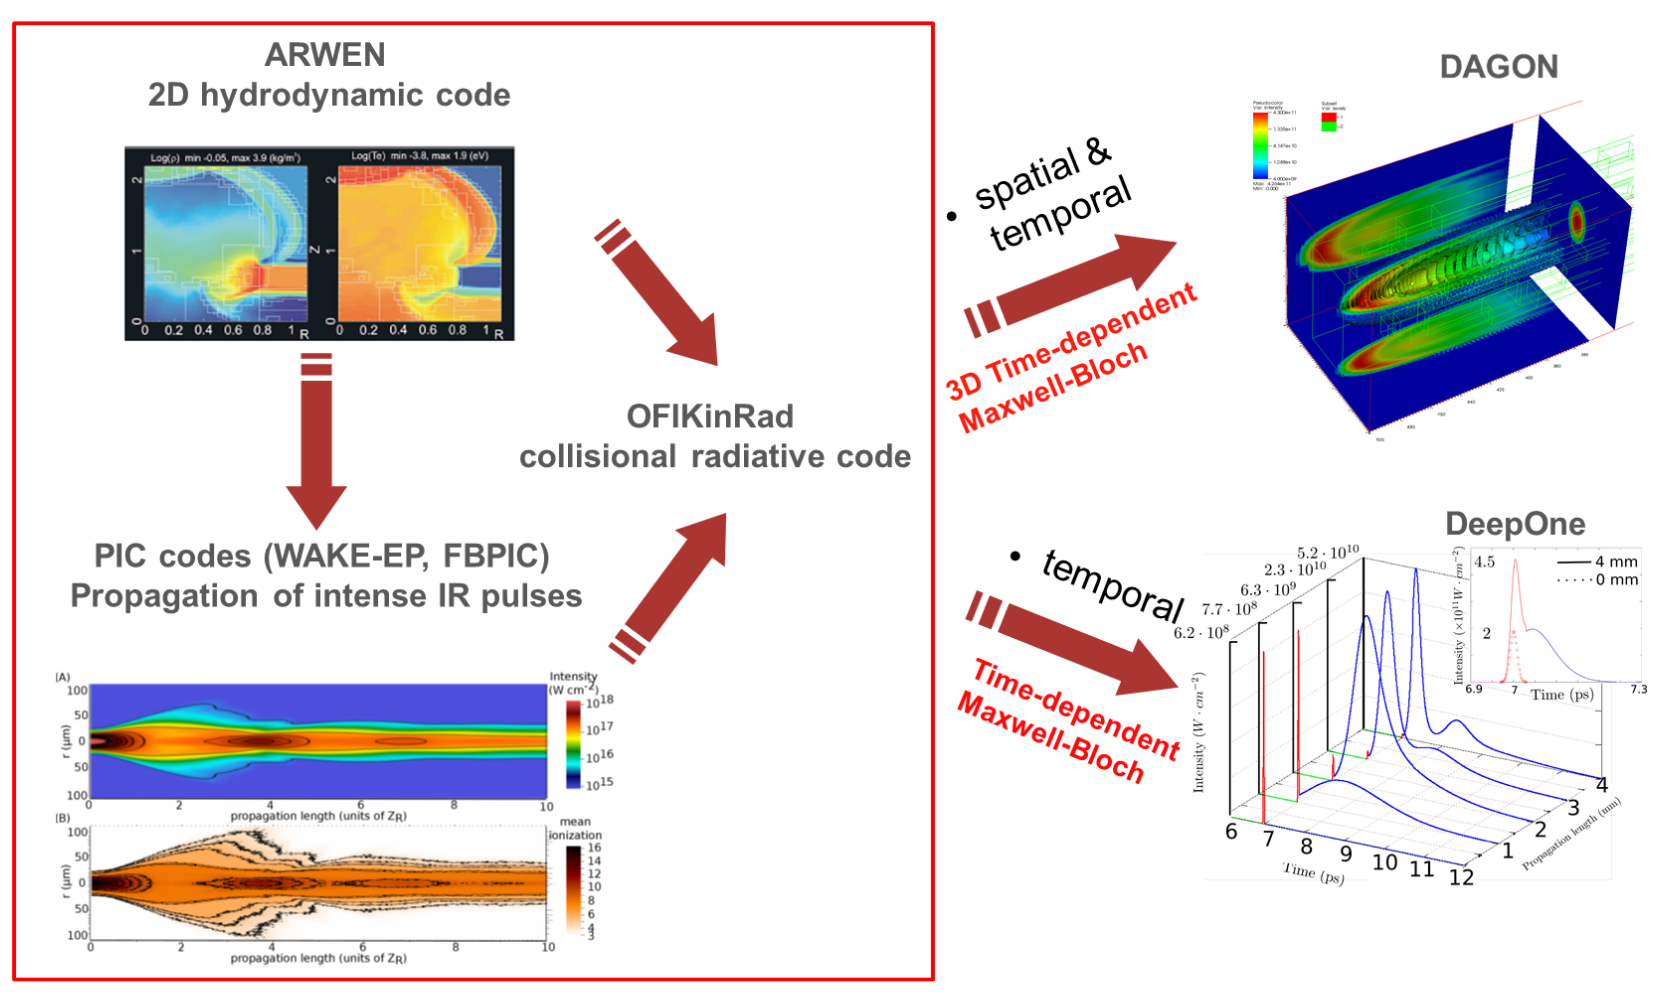
\includegraphics[width=0.8\textwidth]{Figuras/ch3_codig.png}
  \caption{Relaciones de dependencia básicas entre los programas participantes. \autocite{Gil2021}}
  \label{fig:3.2}
\end{figure}

\begin{itemize}

    \item Código ARWEN. Es un código 2D desarrollado en el año $2001$ en el Instituto de Fusión Nuclear \enquote{Guillermo Velarde} (IFN-GV) de la Universidad Politécnica de Madrid\autocite{Ogando2001} para simular con precisión el transporte de radiación y la hidrodinámica durante las etapas posteriores a la compresión del blanco en la fusión por confinamiento inercial\autocite{Velarde2005} o \emph{\acrfull{icf}}, concretamente: la implosión de la cápsula, el precalentamiento y el enfriamiento del material comprimido.

      Su desarrollo también ha permitido, además de estudiar los láseres \acrshort{xuv} basados en plasmas\autocite{Oliva2009,Oliva2010}, modelar la evolución hidrodinámica y colisión de remanentes de supernovas en un medio interestelar homogéneo\autocite{Velarde2006}, proporcionando adicionalmente la capacidad de reproducir en laboratorios ---mediante la ablación láser de un blanco de plástico--- condiciones similares a pequeñas y grandes escalas. 

      Desde una perspectiva matemática, ARWEN introduce como método numérico un esquema de Godunov de segundo orden, permitiendo extraer resultados a cerca de la distribución de electrones o la ionización media en un plasma, necesarios para iniciar la ejecución de los códigos \acrfull{pic} del próximo punto. Las distintas fases de la dinámica de fluidos (convección térmica), transporte electrónico (conducción térmica) y transporte radiativo (radiación térmica) tienen múltiples ecuaciones acopladas, resultando un sistema complejo que necesita resolverse secuencialmente, pero de forma aislada, ilustrado en la Figura \ref{fig:3.3}

      Individualmente, cada módulo utiliza métodos totalmente distintos para encontrar la solución de las ecuaciones correspondientes. Sin embargo, globalmente, están sujetos a una técnica conocida como \emph{Malla Adaptativa Refinada} o \emph{\acrfull{amr}}\autocite{Berger1989,Rendleman2000}. La técnica incrementa los recursos computacionales dedicados a las regiones del dominio de la solución donde los errores de cálculos son más elevados, aumentando el refinamiento (la finura de las particiones del espacio) del mallado del dominio donde el problema presenta mayor dificultad, ya sea la frontera o el interior del mismo.

      \begin{figure}
        \centering
        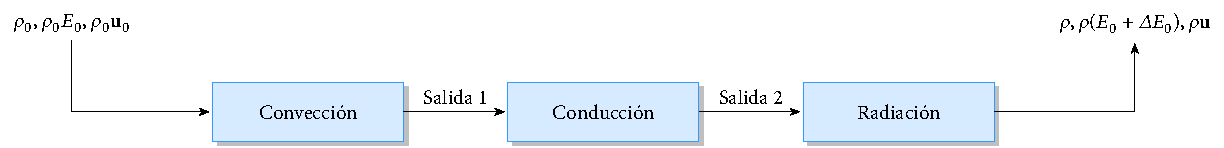
\includegraphics[width=\textwidth]{Figuras/ch3_arwen.pdf}
        \caption{Acoplamiento resuelto numéricamente con el código ARWEN. Adaptado de E. Oliva ($2010$) \autocite{Oliva2010a}}
        \label{fig:3.3}
      \end{figure}

     En problemas que presentan regiones con geometrías complejas, como la formación de ondas de choque en perfiles aerodinámicos, o la interacción de estructuras como supernovas y plasmas astrofísicos a grandes distancias, conseguir tiempos de simulación aceptables es imposible cuando esta técnica no está implementada en el algoritmo de cálculo numérico. Este paradigma está introducido a través del paquete de software libre AMReX\autocite{Zhang2019a}, desarrollado conjuntamente por el \emph{\acrfull{lbnl}}, \emph{\acrfull{nrel}} y \emph{\acrfull{anl}} dentro del marco de un proyecto financiado por el Departamento de Energía de los Estados Unidos.

     Dentro de la temática de este trabajo, la incorporación de una guía de ondas en el plasma amplificador de radiación \acrshort{xuv} necesita utilizar ARWEN para reproducir el comportamiento del plasma\autocite{Oliva2018}, al igual que sucede cuando el blanco que forma el plasma es sólido. En cambio, los esquemas basados exclusivamente en plasmas gaseosos tipo \acrshort{ofi} ---presentados en la sección \S\ref{sec:1.4.2}---, los parámetros físicos mostrados en la sección \S\ref{sec:1.2.1} permanecen aproximadamente constantes a las escalas temporales ($\sim \qty{10}{ps}$) que participan en la amplificación.
    \item Código FBPIC. Los algoritmos \acrfull{pic} están dedicados a resolver fundamentalmente problemas relacionados con plasmas astrofísicos\autocite{Godfrey1974,Kirchen2016}, aunque también han sido empleados en otras áreas de la física. Existen varios códigos basados en este algoritmo, donde el código \emph{\acrfull{fbpic}}\autocite{Lehe2016} es especialmente útil cuando el problema presenta simetría cilíndrica en plasmas de distintas densidades, mientras que otros códigos como WAKE-EP están restringidos a plasmas de baja densidad. Este primer ejemplo, es empleado para estudiar la propagación del pulso \acrshort{nir} de bombeo a través de la columna de plasma originada con anterioridad y, permite estudiar la formación de los iones de kriptón \ce{Kr^{8+}} que amplifican la luz \acrshort{xuv}.

      En analogía directa con el concepto de \enquote{partícula fluida} estudiado en mecánica de fluidos, este código considera el plasma como un conjunto de \enquote{macropartículas} que engloban una gran cantidad de partículas cargadas en su interior ($\sim 10^{20}$ iones y electrones), esto es, tantas como moléculas encierran las partículas fluidas contempladas normalmente en dinámica de fluidos. La macropartícula es escogida como unidad elemental para realizar los cálculos, y determinar los campos eléctricos $\symbfcal{E}$ y magnéticos $\symbfcal{B}$, a partir de las posiciones y velocidades de la macropartícula, y viceversa.

      Naturalmente, las fuentes y los campos están acoplados mediante las ecuaciones de Maxwell, siendo necesario recurrir a un método de cálculo en lazo cerrado, que discretiza el intervalo temporal de la simulación y repite los cálculos en cada subintervalo de la división realizada hasta conseguir la precisión necesaria, como muestra la Figura \ref{fig:3.4}. Además, \acrshort{fbpic} está diseñado para reducir el esfuerzo computacional necesario para simular velocidades relativistas en escenarios tridimensionales, descomponiendo en modos de Fourier los campos electromagnéticos de las macropartículas, o bien, resolviendo las ecuaciones de Maxwell en el espacio de fases.

      \begin{figure}[htbp]
        \centering
        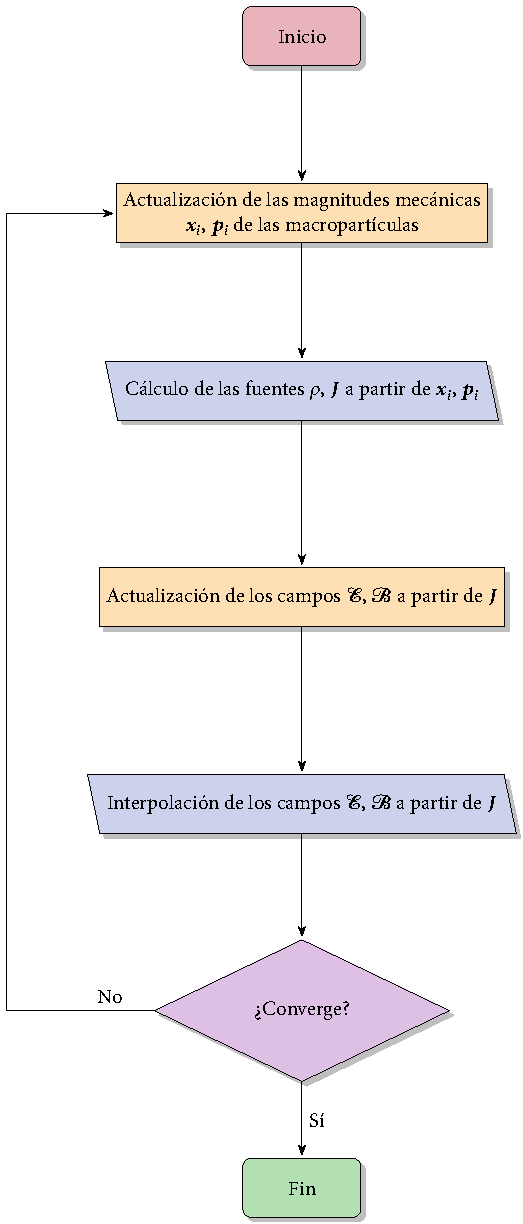
\includegraphics[width=0.4\textwidth]{Figuras/ch3_fbpic.pdf}
        \caption{Diagrama de flujo utilizado por el código \acrshort{fbpic}}
        \label{fig:3.4}
      \end{figure}

    \item Código OFIKinRad. Es un código encargado de estudiar, exclusivamente, la física atómica del plasma amplificador. Recibe como parámetros de entrada la intensidad del pulso \acrshort{nir}, después del primer máximo de intensidad y su focalización por la columna de plasma, la longitud de onda y su polarización, obteniendo como parámetros de salida información fundamental para continuar la simulación del proceso de amplificación, por ejemplo, la temperatura del plasma, las tasas de colisiones entre iones y electrones, o la distribución de los electrones en el canal de plasma.

      Además, la distribución electrónica en el espacio incorpora el perfil de energías de los electrones después de la inyección del pulso \acrshort{nir} inicial, a partir del cual pueden determinarse las tasas de colisiones mencionadas, importantes para resolver las ecuaciones de Maxwell-Bloch descritas durante la sección \S\ref{sec:3.1}. Los iones \ce{Kr^{8+}} son muy masivos ---en comparación con los electrones--- y sus choques apenas modifican la distribución de energías de los electrones. Sin embargo, las colisiones entre electrones multiplican la distribución de energías por un factor de escala, cambiando también la forma del perfil, mientras que las colisiones ión-electrón repercuten en la densidad de electrones y sus energías medias.

      Los niveles de energía contemplados en el código se corresponden únicamente con el ión de kriptón \ce{Kr^{8+}}, responsable del efecto láser que amplifica la radiación \acrshort{xuv}. También calcula las probabilidades de ionización y excitación asociadas al kriptón (las secciones eficaces microscópicas), necesarias también a la hora de predecir la dinámica temporal del perfil de energías de los electrones mediante la ecuación de transporte de Boltzmann. En última instancia, el código determina la inversión poblacional conseguida y su evolución en el tiempo, es decir, la ganancia del medio.
    \item Código Dagon. Está escrito específicamente para modelar y simular la amplificación de láseres \acrshort{sxrl} basados en plasmas calientes y densos. Como mostraba la sección \S\ref{sec:3.1}, resuelve las ecuaciones de Maxwell-Bloch (\acrshort{mbe}) en tres dimensiones introduciendo algunas hipótesis de partida, partiendo de los parámetros de salida obtenidos mediante OFIKinRad, como la frecuencia de las colisiones entre iones y electrones, los niveles poblacionales de la transición láser, o la densidad electrónica de la preforma de plasma.
      
      Apareció en el Instituto de Fusión Nuclear \enquote{Guillermo Velarde} (IFN-GV)\autocite{Oliva2017}, dentro de un proyecto respaldado por el Ministerio de Educación, Cultura y Deporte de España a través del programa de investigación \enquote{Plan Nacional}, el programa \emph{People Programme} (\emph{Marie Curie Actions}) de la Unión Europea (FP7/\numrange{2007}{2013}) bajo el Acuerdo de Subvención de la Agencia Ejecutiva de Investigación (REA), y el programa de investigación e innovación \emph{Horizon 2020} de la Unión Europea. Su misión principal es reproducir satisfactoriamente la amplificación de \acrshortpl{hoh} cuando las heterogeneidades presentes en el plasma impedían conseguir una descripción precisa del proceso, como ocurría con códigos anteriores como COLAX (código bidimensional)\autocite{Larroche2000,Almiev2007} o DeepOne (código unidimensional, precursor de Dagon)\autocite{Oliva2011}.

      Una vez resueltas las ecuaciones diferenciales para el campo eléctrico, polarización y los niveles poblacionales, la información de salida es dirigida a programas de postprocesamiento como VisIt que permiten representar y visualizar estos resultados. En este trabajo, la utilización de Dagon es fundamental para estudiar en tres dimensiones la evolución temporal del armónico inyectado a través de la columna de plasma.

\end{itemize}

En resumen, las diferentes escalas y fenómenos físicos que participan en los \acrshort{sxrl} basados en plasmas exige emplear múltiples códigos acoplados entre sí, desarrollados para el modelado matemático y la comprensión de distintos aspectos como la propagación del haz infrarrojo o la amplificación de la semilla de armónicos de alto orden.

\begin{footheorem*}{Esquema computacional}

  \begin{enumerate}

        \item La hidrodinámica del plasma es estudiada mediante el código 2D ARWEN, encargado del transporte de energía mediante conducción, convección y radiación.
        \item La propagación de pulsos infrarrojos intensos a través del plasma es modelada mediante el código 2D FBPIC, empleado en física de plasmas relativistas.
        \item La abundancia de iones, poblaciones, tasas de colisiones, etc., se calcula mediante el código 0D OFIKinRad, encargado de caracterizar el plasma amplificador.
        \item La amplificación de armónicos de alto orden en plasmas es calculada mediante el código 3D Dagon, encargado de implementar el modelo de Maxwell-Bloch.

  \end{enumerate}

\end{footheorem*}

\section{Esquema experimental}\label{sec:3.3}
La ejecución del experimento y los detalles básicos de los instrumentos utilizados tienen un papel fundamental en las simulaciones llevadas a cabo en este proyecto. En el plano histórico, este proyecto forma parte de una línea de investigación que, a su vez, tiene su origen en una serie de experimentos realizados en el \emph{\acrfull{loa}} en colaboración con investigadores del Instituto de Fusión Nuclear \enquote{Guillermo Velarde} (IFN-GV), entre otros grupos alrededor del mundo. Este esfuerzo conjunto ha conseguido alcanzar hitos como la obtención de \acrshortpl{hoh} amplificados con duraciones de femtosegundos, o la demostración de la diagnosis de plasmas mediante la medición de la fase e intensidad del armónico amplificado\autocite{Depresseux2015,Tuitje2020}.

Este laboratorio es un centro de investigación mixto formado por el \emph{\acrfull{cnrs}}, la \emph{\acrfull{ep}} y la \emph{\acrfull{ensta}}, ubicado en el interior del campus sur de la \acrshort{ep}, en Palaiseau, Francia. Los campos de investigación tratados en su interior abarcan múltiples áreas relacionadas con la óptica de láseres-plasmas ultrarrápidos, entre los cuales se encuentra la puesta en marcha, operación, modelización y simulación del láser \acrshort{sxrl} basado en un plasma de iones \ce{Kr^{8+}}, centro de estudio de este trabajo.

Las instalaciones que albergan la infraestructura (ver Figura \ref{fig:3.5}) donde el experimento fue realizado inicialmente están dentro de una gran habitación llamada \emph{Salle Jaune} (una sala amarilla), donde un sistema láser \ce{Ti{:}Zafiro} ---un cristal de zafiro (\ce{Al2O3}) dopado con iones de titanio \ce{Ti^{3+} neonoide}--- tiene la función de generar todos los pulsos necesarios. El sistema, con \qty{120}{TW} de potencia, repartidos en dos canales de \qty{60}{TW}, posee seis líneas láser sincronizadas con capacidad para generar pulsos de \qty{30}{fs}, de las cuales tres están dedicadas a la aceleración de electrones y generación de rayos X.

En el esquema seguido para conseguir amplificar la semilla \acrshort{hoh} pueden distinguirse cuatro fases:

\begin{enumerate}

    \item En primer lugar, un primer pulso láser penetra sobre un chorro de gas de kriptón de alta densidad, depositando la energía necesaria para ionizar rápidamente los átomos y producir la inversión poblacional requerida mediante colisiones con los electrones producidos. Es una secuencia formada por los efectos de la ionización de efecto túnel (\acrshort{ofi}) y excitación colisional, desarrollados durante el capítulo \S\ref{cap:1}.
    \item En segundo lugar, comienza la preparación para inyectar la semilla de armónicos de alto orden (\acrshortpl{hoh}) para su amplificación. Las elevadas densidades electrónicas utilizadas, en torno a aproximadamente \qtyrange{e19}{e20}{cm^{-3}}\autocite{Tuitje2020}, y próximas a la densidad crítica ($\simeq \qty{e21}{cm^{-3}}$) para la frecuencia de la radiación \acrshort{xuv}, provocan un desenfoque de la semilla que disminuye la distancia de propagación recorrida, reduciendo drásticamente la longitud efectiva del medio y, por tanto, la ganancia conseguida.

      Como solución a este problema, se introduce una columna de plasma que actúa como guía de ondas de la semilla\autocite{Depresseux2015}. En la Figura \ref{fig:3.6}, aparece la secuencia de pulsos utilizados para crear la preforma de plasma. Primero, un pulso infrarrojo ($\lambda = \qty{800}{nm}$) llamado \enquote{cebador} o \emph{ignitor} (\qty{130}{mJ}, \qty{30}{fs}) forma el canal de plasma y, inmediatamente después (con \qty{600}{ps} de retraso), otro pulso infrarrojo denominado \enquote{calentador} o \emph{heater} (\qty{690}{mJ}, \qty{600}{ps}) calienta los electrones. De esta manera, se produce una expansión hidrodinámica que induce un gradiente de densidad electrónica creciente en la dirección radial de la columna de plasma, permitiendo enfocar el haz de armónicos cuando comienza a desenfocarse.

      \begin{figure}[htbp]
        \centering
        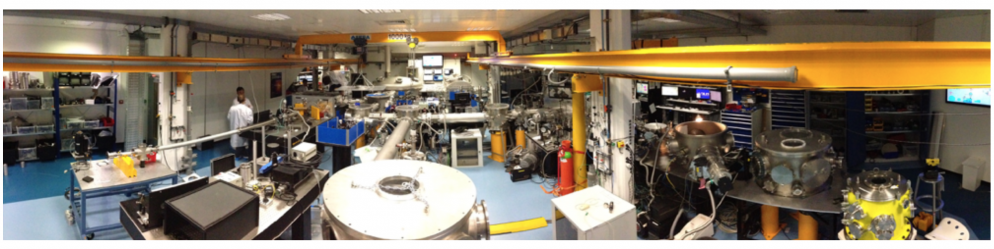
\includegraphics[width=\textwidth]{Figuras/ch3_sallejaune.png}
        \caption{Sistema láser \emph{Salle Jaune} del \acrshort{loa} utilizado para la amplificación de láseres \acrshort{sxrl} basados en plasmas. Salle Jaune. Laboratoire d'Optique Apliquée. \url{https://loa.ensta-paris.fr/fr/le-laboratoire/infrastructures-experimentales/salle-jaune/}.}
        \label{fig:3.5}
      \end{figure}
    \item En tercer lugar, una vez preparado el canal de plasma para el guiado de los pulsos, un tercer pulso infrarrojo de bombeo (\qty{1.36}{J}, \qty{30}{fs}) es enfocado en la entrada del canal mediante un espejo esférico, transfiriendo parte de su energía para producir el ión \ce{Kr^{8+}}, responsable de la transición láser, y calentando los electrones encargados de producir la inversión de población mediante choques ión-electrón. En resumen, esta etapa del proceso está basada en el bombeo colisional producido por un haz infrarrojo.
    \item Finalmente, un cuarto pulso láser infrarrojo (\qty{16}{mJ}, \qty{350}{fs}) es obligado a pasar a través de una celda llena gas argón a alta presión. La fuerte interacción no lineal de ambos genera el armónico de alto orden deseado (\acrshort{hhg}), en este experimento, el modo número $25$, multiplicando su energía y manteniendo las propiedades ópticas excelentes del \acrshort{hoh} generado. Visualmente, la Figura \ref{fig:3.6} muestra un esquema de todas las etapas presentadas, obteniendo la emisión \acrshort{sxrl} buscada.

\end{enumerate}

\begin{figure}[htbp]
  \centering
  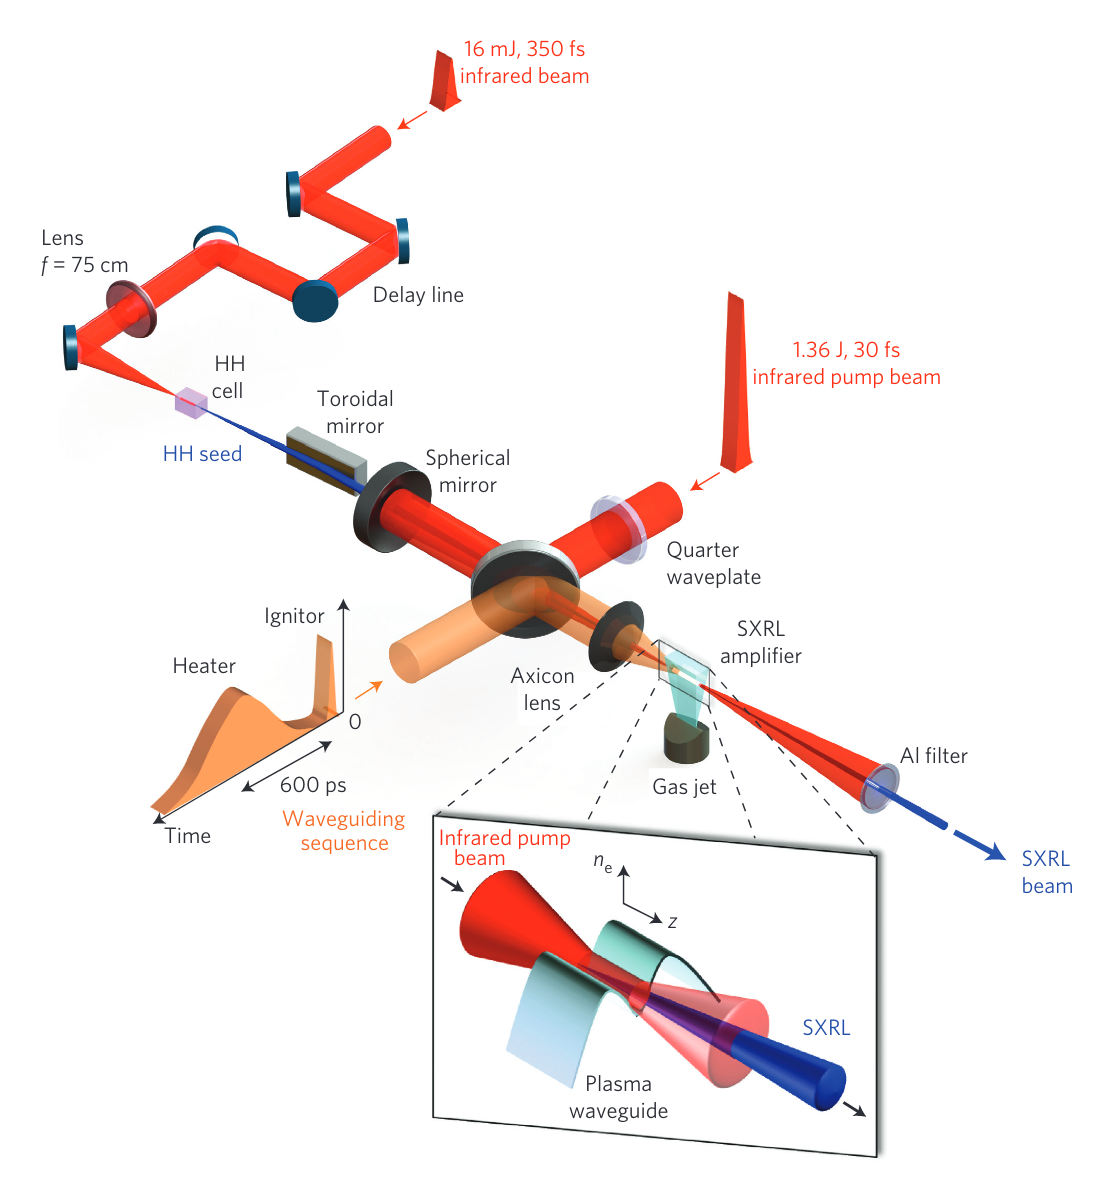
\includegraphics[width=0.6\textwidth]{Figuras/ch3_exper1.png}
  \caption{Esquema de la disposición experimental\autocite{Depresseux2015} utilizada para la amplificación del láser \acrshort{sxrl}. Un filtro de aluminio elimina la radiación infrarroja sobrante, permitiendo analizar la emisión amplificada posteriormente.}
  \label{fig:3.6}
\end{figure}

Posteriormente, la radiación \acrshort{xuv} es enfocada sobre una muestra (un patrón de agujeros dispuestos de forma periódica) mediante un sistema de espejos multicapa\autocite{Tuitje2020}, pasando previamente por un sistema de filtros de aluminio que bloquean la radiación \acrshort{nir} residual. La reconstrucción de los perfiles de intensidad y fase analizados en este Trabajo Fin de Máster, puede conseguirse en el laboratorio empleando una técnica computacional llamada \emph{pticografía}, que permite escanear y registrar ---mediante un detector \acrshort{ccd}--- los patrones de difracción formados en la muestra agujereada. La superposición de estos patrones permite recuperar la amplitud compleja de la intensidad del haz láser \acrshort{sxrl}, mostrada en la Figura \ref{fig:3.7}.

\begin{figure}[htbp]
  \centering
  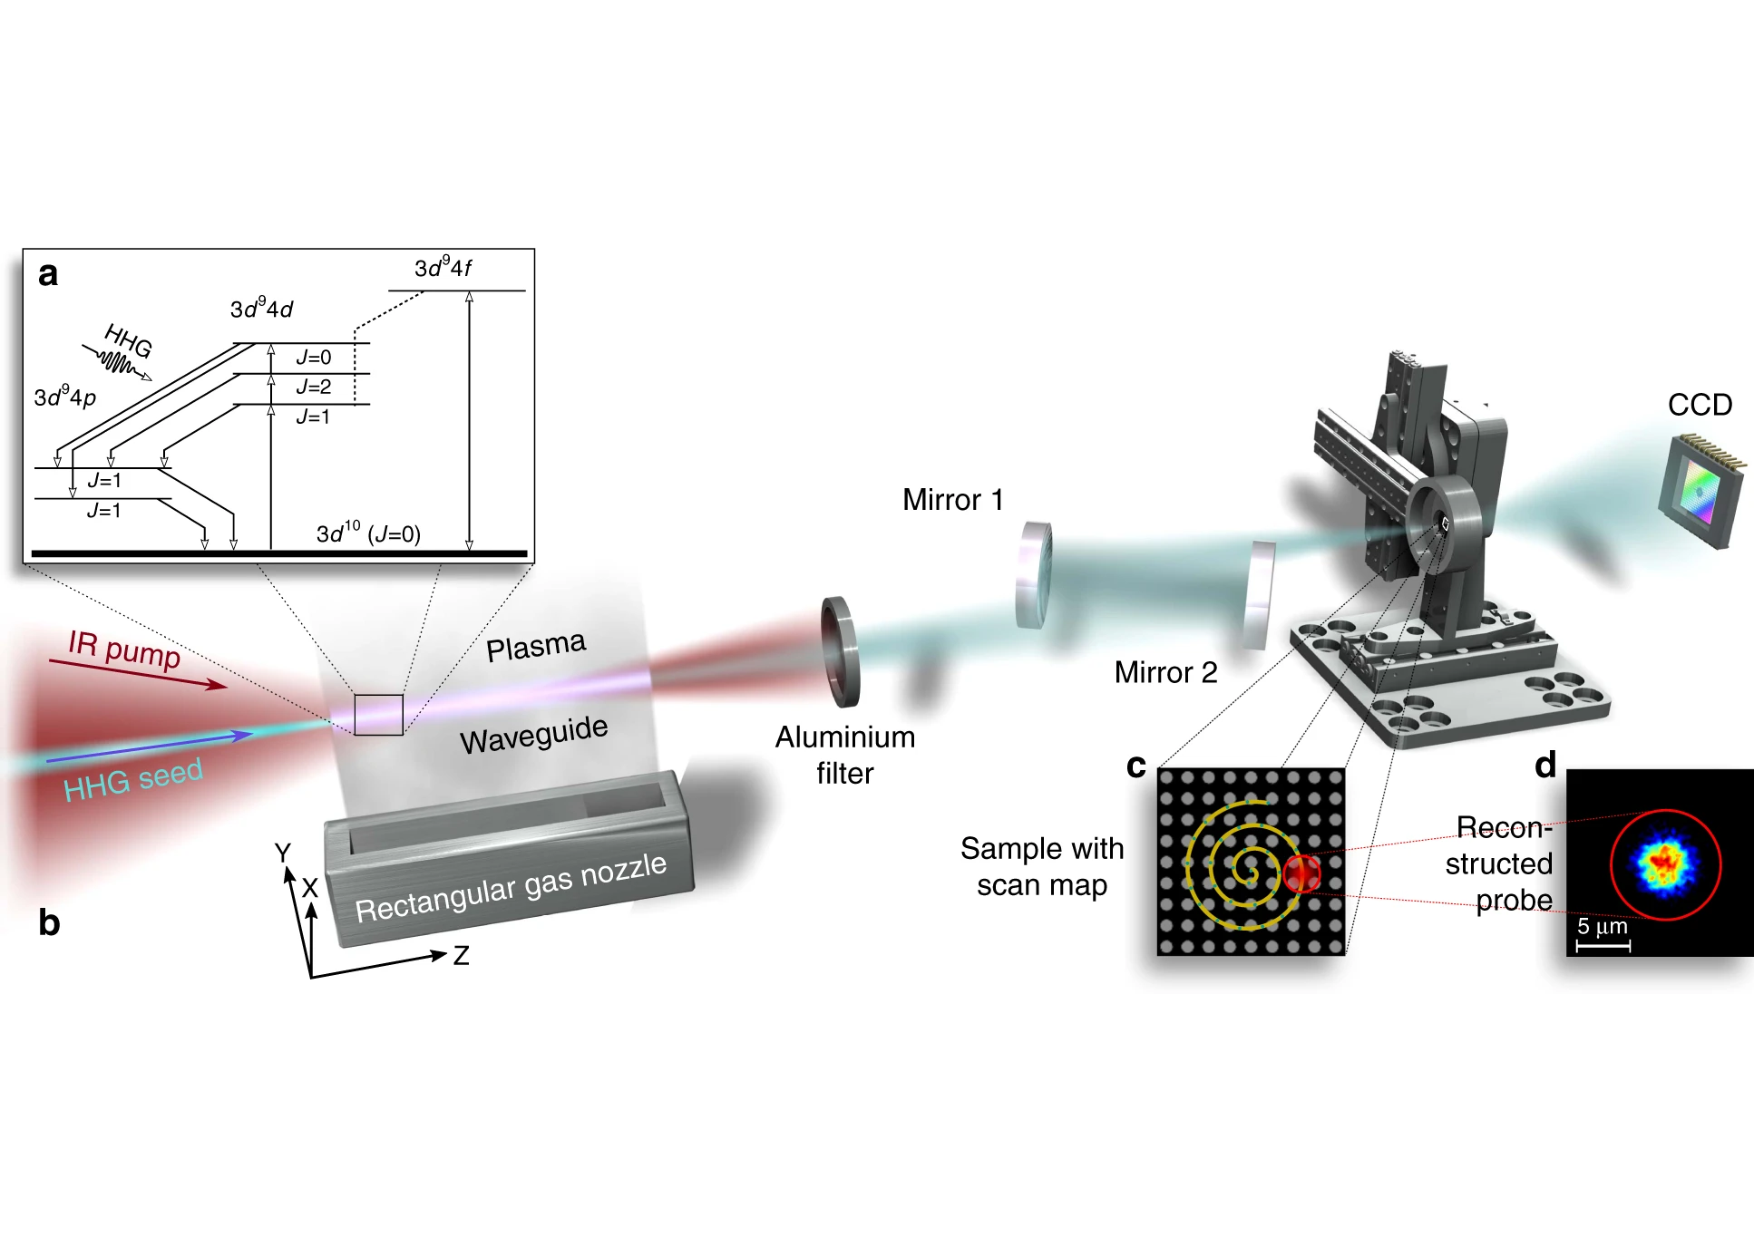
\includegraphics[width=0.8\textwidth]{Figuras/ch3_exper2.pdf}
  \caption{Esquema de los elementos\autocite{Tuitje2020} utilizados para la diagnosis láser-plasma. \textbf{c}, La radiación emitida es dirigida hacia una muestra para registrar el patrón de difracción. \textbf{d}, Amplitud compleja de la intensidad reconstruida mediante pticografía.}
  \label{fig:3.7}
\end{figure}

Así, conocidos los fundamentos físicos y los experimentos realizados hasta el momento, es posible comenzar a explicar los parámetros principales empleados en Dagon, e introducir o modificar pequeños fragmentos del código. De esta forma, tal y como aparecía en el capítulo \S\ref{cap:2}, pueden analizarse las consecuencias de implementar estos cambios y su adecuación con las observaciones experimentales.

\section{Parámetros de las simulaciones}\label{sec:3.4}
Los parámetros iniciales empleados en Dagon reflejan una situación inicial donde la preforma de plasma está generada, es decir, la secuencia cebador-calentador ha ocurrido, a la espera del haz \acrshort{nir} de bombeo y la inyección de la semilla \acrshort{hoh} para su amplificación. Concretamente, el escenario de partida consiste en un plasma homogéneo de iones \ce{Kr^{3+}} (el grado de ionización al comienzo de la simulación) con una densidad atómica de neutros $n_{0} = \qty{9.875e17}{cm^{-3}}$. El perfil radial de densidad de la preforma óptica de plasma está dado por
\begin{equation}\label{eq:3.18}
  N_{Kr} =   
  \begin{cases}
    1 + (r/r_{0})^{2}, & \text{si $r<r_{0}$},\\
    \left[1 + (r_{c}/r_{0})^{2}\right]^{\frac{r_{v}-r}{r_{v}-r_{c}}}, & \text{si $r\ge r_{0}$},
  \end{cases}
\end{equation}
donde $r_{c} = \qty{38}{µm}$ es el radio del canal de plasma, y los parámetros $r_{0} = \qty{80}{µm}$, $r_{v} = \qty{90}{µm}$ controlan la forma parabólica de la densidad de neutros. Esta función permite modelar el perfil parabólico creciente con el radio producido por la secuencia de pulsos infrarrojos mencionada, y la desaparición de los iones a partir de un determinado radio del canal $r_{c}$.

A lo largo de la longitud del canal ($z_{0} = \qty{5}{mm}$) de plasma, representado por una celda de \qtyproduct{5000 x 100 x 100}{mm}, la intensidad del pulso láser de bombeo disminuye con la distancia recorrida, además de presentar la forma de una distribución Gaussiana en dirección radial. Adicionalmente, los experimentos observaron una sobreionización\autocite{Tuitje2020} a la entrada (la intensidad máxima es alcanzada a la entrada del canal) y en la región intermedia de la columna de plasma (debido al fenómeno de focalización producido durante el guiado). A raíz de estos sucesos, la densidad de iones \ce{Kr^{8+}} disminuye y la densidad de electrones aumenta en ambas regiones.

Las funciones de densidad implementadas en las simulaciones para la modelización de estos fenómenos, antes de comenzar el proceso de modificación y estudio de los parámetros, que ocupará el capítulo \S\ref{cap:4}, siguen las expresiones
\begin{align}
  \label{eq:3.19a}
  N_{Kr^{8+}} &= N_{Kr}\frac{\eu^{-\frac{(\max(r,r_{L}))^{2}}{2 \sigma_{rL}^{2}}}}{\eu^{-\frac{r_{L}^{2}}{2 \sigma_{rL}^{2}}}}\left(1-\eu^{-\frac{(z-\mathtt{zshift}*z_{0})^{2}}{2 \sigma_{z}^{2}}}\eu^{-\frac{r^{2}}{2 \sigma_{r}^{2}}}\right)\left(1-\eu^{-\frac{z^{2}}{2 \sigma_{z0}^{2}}}\frac{\eu^{-\frac{(\max(r,r_{L0}))^{2}}{2 \sigma_{r0}^{2}}}}{\eu^{-\frac{r_{L0}^{2}}{2 \sigma_{r0}^{2}}}}\right), \\
  \label{eq:3.19b}
  n_{e} &= N_{Kr}\left(1+\mathtt{cen\_fac}*\eu^{-\frac{(z-\mathtt{zshift}*z_{0})^{2}}{2 \sigma_{z}^{2}}}\eu^{-\frac{r^{2}}{2 \sigma_{r}^{2}}}\right)+\mathtt{z0\_fac}*\eu^{-\frac{z^{2}}{2 \sigma_{z0}^{2}}}\eu^{-\frac{r^{2}}{2 \sigma_{r0}^{2}}},
\end{align}
donde $\mathtt{zshift}$ es un parámetro introducido para controlar la posición de la región intermedia sobreionizada, y $\mathtt{cen\_fac}$, $\mathtt{z0\_fac}$ son factores de escala que regulan la magnitud de la densidad electrónica en las regiones sobreionizadas. 

Por otra parte, las variables $z$, $r$ representan la longitud recorrida por la semilla y el radio del canal, respectivamente, mientras que las dispersiones de cada dimensión están representadas mediante los parámetros $\sigma_{r,z}$ asociadas a cada variable. Los parámetros más importantes, que serán constantemente modificados y objeto de estudio durante el próximo capítulo \S\ref{cap:4}, son $r_{L} = \qty{5}{µm}$ y $\sigma_{rL} = \qty{15}{µm}$: el radio de anchura del canal con abundancia de iones \ce{Kr^{8+}} y su dispersión Gaussiana asociada, respectivamente. De este modo, delimitan la región del canal con presencia del ión amplificador suponiendo una distribución constante a lo largo de toda la celda. 

Esta hipótesis, es el sujeto principal al comienzo de las modificaciones realizadas en este proyecto, introduciendo un ancho variable con la longitud del canal $z$ que represente, de forma aproximada, la región donde se encuentran los iones \ce{Kr^{8+}}. Los perfiles utilizados para sustituir estos valores homogéneos están expresados por \emph{curvas logísticas} o \emph{sigmoides}, que aparecerán detallados en la sección \S\ref{sec:4.1}. 

También existen datos de entrada en Dagon relacionados con el dominio simulado, como las dimensiones (\texttt{domain\_length}, \texttt{domain\_width}, y el número de celdas en cada eje \texttt{cell\_number\_x}, \texttt{cell\_number\_y} y \texttt{cell\_number\_z}), las particiones espaciales del mallado (\texttt{ghost\_cell\_x}, \texttt{ghost\_cell\_y} y \texttt{ghost\_cell\_z}), o la discretización temporal del intervalo (las condiciones iniciales \texttt{init\_time}, \texttt{end\_time}, y la finura de la partición \texttt{init\_dt}); el pulso \acrshort{nir} de bombeo, como la duración del pulso (\texttt{tauIR}), la longitud de onda (\texttt{IRlambda}), o el tiempo de retardo respecto de la inyección de la semilla (\texttt{tcentIR}); y la semilla de armónicos de alto orden (\acrshort{hoh}), como el instante de inyección (\texttt{tcent}), la energía (\texttt{energy}), o la amplitud (\texttt{fwhmx} y \texttt{fwhmy}).

La Tabla \ref{tab:3.1} recoge los parámetros más importantes que se han mencionado, recogidos en un archivo secundario auxiliar, cargados en Dagon a través de una subrutina que realiza una llamada a dicho archivo.

\begin{table}[htpb]
  \centering
  \scriptsize
  \caption{Condiciones iniciales utilizadas en un archivo ASCII para alimentar a Dagon. Parámetros en unidades del Sistema Internacional de unidades.}
  \label{tab:3.1}
  \begin{tabular}{lSlSlS}
  \toprule
  \multicolumn{2}{c}{{Dominio}} & \multicolumn{2}{c}{{Semilla HOH}} & \multicolumn{2}{c}{{Láser NIR}}                                                                                          \\ 
  \cmidrule{1-2}\cmidrule(l){3-4}\cmidrule(l){5-6}
  \multicolumn{1}{c}{{Nombre}}  & \multicolumn{1}{c}{{Valor}}  & \multicolumn{1}{c}{{Nombre}} & \multicolumn{1}{c}{{Valor}} & \multicolumn{1}{c}{{Nombre}} & \multicolumn{1}{c}{{Valor}}            \\
  \midrule
  \texttt{in\_time}              & 0            & \texttt{tcent}  & 0,2e-12 & \texttt{tcentIR}  & 150e-15                                                                                                  \\ 
  \texttt{end\_time}             & 18e-12       & \texttt{fwhm}   & 100e-15 & \texttt{tauIR}    & 30e-15                                                                                                  \\ 
  \texttt{init\_dt}              & 0,01e-12     & \texttt{energy} & 1e-9    & \texttt{IRlambda} & 800e-9                                                                                                   \\ 
  \texttt{domain\_length}        & 5e-3         & \texttt{fwhmx}  & 25e-6    & &                                                                                                   \\ 
  \texttt{domain\_width}         & 100e-6       & \texttt{fwhmy}  & 25e-6    & &                        \\ 
  \texttt{cell\_number\_(x,y,z)} & \numproduct{1000 x 100 x 100}  &          & & &                      \\ 
  \texttt{ghost\_cell\_(x,y,z)}  & \numproduct{6 x 2 x 2}         &          & & &                      \\ 
  \bottomrule
  \end{tabular}
\end{table}
